% Options for packages loaded elsewhere
\PassOptionsToPackage{unicode}{hyperref}
\PassOptionsToPackage{hyphens}{url}
%
\documentclass[
  12pt,
  a4paper,
]{scrreprt}
\usepackage{amsmath,amssymb}
\usepackage{setspace}
\usepackage{iftex}
\ifPDFTeX
  \usepackage[T1]{fontenc}
  \usepackage[utf8]{inputenc}
  \usepackage{textcomp} % provide euro and other symbols
\else % if luatex or xetex
  \usepackage{unicode-math} % this also loads fontspec
  \defaultfontfeatures{Scale=MatchLowercase}
  \defaultfontfeatures[\rmfamily]{Ligatures=TeX,Scale=1}
\fi
\usepackage{lmodern}
\ifPDFTeX\else
  % xetex/luatex font selection
  \setmainfont[Ligatures=TeX]{PT Serif}
  \setsansfont[Ligatures=TeX,Scale=MatchLowercase]{PT Sans}
  \setmonofont[Scale=MatchLowercase,Scale=0.9]{PT Mono}
\fi
% Use upquote if available, for straight quotes in verbatim environments
\IfFileExists{upquote.sty}{\usepackage{upquote}}{}
\IfFileExists{microtype.sty}{% use microtype if available
  \usepackage[]{microtype}
  \UseMicrotypeSet[protrusion]{basicmath} % disable protrusion for tt fonts
}{}
\usepackage{xcolor}
\usepackage{graphicx}
\makeatletter
\def\maxwidth{\ifdim\Gin@nat@width>\linewidth\linewidth\else\Gin@nat@width\fi}
\def\maxheight{\ifdim\Gin@nat@height>\textheight\textheight\else\Gin@nat@height\fi}
\makeatother
% Scale images if necessary, so that they will not overflow the page
% margins by default, and it is still possible to overwrite the defaults
% using explicit options in \includegraphics[width, height, ...]{}
\setkeys{Gin}{width=\maxwidth,height=\maxheight,keepaspectratio}
% Set default figure placement to htbp
\makeatletter
\def\fps@figure{htbp}
\makeatother
\setlength{\emergencystretch}{3em} % prevent overfull lines
\providecommand{\tightlist}{%
  \setlength{\itemsep}{0pt}\setlength{\parskip}{0pt}}
\setcounter{secnumdepth}{5}
\newlength{\cslhangindent}
\setlength{\cslhangindent}{1.5em}
\newlength{\csllabelwidth}
\setlength{\csllabelwidth}{3em}
\newlength{\cslentryspacingunit} % times entry-spacing
\setlength{\cslentryspacingunit}{\parskip}
\newenvironment{CSLReferences}[2] % #1 hanging-ident, #2 entry spacing
 {% don't indent paragraphs
  \setlength{\parindent}{0pt}
  % turn on hanging indent if param 1 is 1
  \ifodd #1
  \let\oldpar\par
  \def\par{\hangindent=\cslhangindent\oldpar}
  \fi
  % set entry spacing
  \setlength{\parskip}{#2\cslentryspacingunit}
 }%
 {}
\usepackage{calc}
\newcommand{\CSLBlock}[1]{#1\hfill\break}
\newcommand{\CSLLeftMargin}[1]{\parbox[t]{\csllabelwidth}{#1}}
\newcommand{\CSLRightInline}[1]{\parbox[t]{\linewidth - \csllabelwidth}{#1}\break}
\newcommand{\CSLIndent}[1]{\hspace{\cslhangindent}#1}
\ifLuaTeX
\usepackage[bidi=basic]{babel}
\else
\usepackage[bidi=default]{babel}
\fi
\babelprovide[main,import]{russian}
\ifPDFTeX
\else
\babelfont[russian]{rm}{PT Serif}
\fi
\babelprovide[import]{english}
% get rid of language-specific shorthands (see #6817):
\let\LanguageShortHands\languageshorthands
\def\languageshorthands#1{}
\usepackage{indentfirst}
\usepackage{float}
\floatplacement{figure}{H}
\ifLuaTeX
  \usepackage{selnolig}  % disable illegal ligatures
\fi
\usepackage[style=gost-numeric,parentracker=true,backend=biber,hyperref=auto,language=auto,autolang=other*,citestyle=gost-numeric]{biblatex}
\addbibresource{bib/cite.bib}
\IfFileExists{bookmark.sty}{\usepackage{bookmark}}{\usepackage{hyperref}}
\IfFileExists{xurl.sty}{\usepackage{xurl}}{} % add URL line breaks if available
\urlstyle{same}
\hypersetup{
  pdftitle={Отчет по лабораторной работе №5},
  pdfauthor={Выполнила: Афтаева Ксения Васильевна},
  pdflang={ru-RU},
  hidelinks,
  pdfcreator={LaTeX via pandoc}}

\title{Отчет по лабораторной работе №5}
\usepackage{etoolbox}
\makeatletter
\providecommand{\subtitle}[1]{% add subtitle to \maketitle
  \apptocmd{\@title}{\par {\large #1 \par}}{}{}
}
\makeatother
\subtitle{Дисциплина: Математическое моделирование}
\author{Выполнила: Афтаева Ксения Васильевна}
\date{}

\begin{document}
\maketitle

\renewcommand*\contentsname{Содержание}
{
\setcounter{tocdepth}{2}
\tableofcontents
}
\listoffigures
\listoftables
\setstretch{1.5}
\hypertarget{ux446ux435ux43bux44c-ux440ux430ux431ux43eux442ux44b}{%
\chapter{Цель
работы}\label{ux446ux435ux43bux44c-ux440ux430ux431ux43eux442ux44b}}

Рассмотреть простейшую модель взаимодействия двух видов типа «хищник —
жертва» - модель Лотки-Вольтерры. Выполнить задание согласно варианту:
построить график зависимости численности хищников от численности жертв,
а также графики изменения численности хищников и численности жертв при
заданных начальных условиях, найти стационарное сосотояние системы.

\hypertarget{ux437ux430ux434ux430ux43dux438ux435}{%
\chapter{Задание}\label{ux437ux430ux434ux430ux43dux438ux435}}

\textbf{Вариант № 10}:

Для модели «хищник-жертва»:

\begin{equation}
   \begin{cases}
     \frac{dx}{dt} = -0.22x(t)+0.051x(t)y(t)
     \\
     \frac{dy}{dt} = 0.33y(t)-0.041x(t)y(t)
   \end{cases}
\label{eq:01}\end{equation}

Постройте график зависимости численности хищников от численности жертв,
а также графики изменения численности хищников и численности жертв при
следующих начальных условиях: \(x_0 = 3\), \(y_0 = 8\). Найдите
стационарное состояние системы.

\hypertarget{ux442ux435ux43eux440ux435ux442ux438ux447ux435ux441ux43aux43eux435-ux432ux432ux435ux434ux435ux43dux438ux435}{%
\chapter{Теоретическое
введение}\label{ux442ux435ux43eux440ux435ux442ux438ux447ux435ux441ux43aux43eux435-ux432ux432ux435ux434ux435ux43dux438ux435}}

Впервые модель «хищник – жертва» была получена А. Лоткой в 1925 году,
который использовал ее для описания динамики взаимодействующих
биологических популяций. В 1926 году независимо от Лотки аналогичные (к
тому же более сложные) модели были разработаны итальянским математиком
В. Вольтерра {[}1{]}.

В 1931 году Вито Вольтеррой были выведены следующие законы отношения
хищник-жертва:

\begin{itemize}
\item
  закон периодического цикла – процесс уничтожения жертвы хищником
  нередко приводит к периодическим колебаниям численности популяций
  обоих видов, зависящим только от скорости роста плотоядных и
  растительноядных, и от исходного соотношения их численности;
\item
  закон сохранения средних величин – средняя численность каждого вида
  постоянна, независимо от начального уровня, при условии, что
  специфические скорости увеличения численности популяций, а также
  эффективность хищничества постоянны;
\item
  закон нарушения средних величин – при сокращении обоих видов
  пропорционально их числу, средняя численность популяции жертвы растет,
  а хищников – падает {[}2{]}.
\end{itemize}

\textbf{Модель хищник-жертва} – это особая взаимосвязь хищника с
жертвой, в результате которой выигрывают оба. Выживают наиболее здоровые
и приспособленные особи к условиям среды обитания, т.е. все это
происходит благодаря естественному отбору. В той среде где нет
возможности для размножения, хищник рано или поздно уничтожит популяцию
жертвы, в последствии чего вымрет и сам.

Данная двувидовая модель основывается на следующих предположениях:

\begin{itemize}
\item
  численность популяции жертв \(y\) и хищников \(x\) зависят только от
  времени (модель не учитывает пространственное распределение популяции
  на занимаемой территории);
\item
  в отсутствии взаимодействия численность видов изменяется по модели
  Мальтуса, при этом число жертв увеличивается, а число хищников падает;
\item
  естественная смертность жертвы и естественная рождаемость хищника
  считаются несущественными;
\item
  эффект насыщения численности обеих популяций не учитывается;
\item
  скорость роста численности жертв уменьшается пропорционально
  численности хищников {[}3{]}.
\end{itemize}

\begin{equation}
   \begin{cases}
     \frac{dx}{dt} = -ax(t)+bx(t)y(t)
     \\
     \frac{dy}{dt} = cy(t)-dx(t)y(t)
   \end{cases}
\label{eq:02}\end{equation}

В этой модели \(x\) – число хищников, \(y\) - число жертв. Коэффициент
\(c\) описывает скорость естественного прироста числа жертв в отсутствие
хищников, \(a\) - естественное вымирание хищников, лишенных пищи в виде
жертв. Вероятность взаимодействия жертвы и хищника считается
пропорциональной как количеству жертв, так и числу самих хищников
(\(xy\)). Каждый акт взаимодействия уменьшает популяцию жертв, но
способствует увеличению популяции хищников (члены \(dxy\) и \(-bxy\) в
правой части уравнения) {[}3{]}.

\begin{figure}
\hypertarget{fig:001}{%
\centering
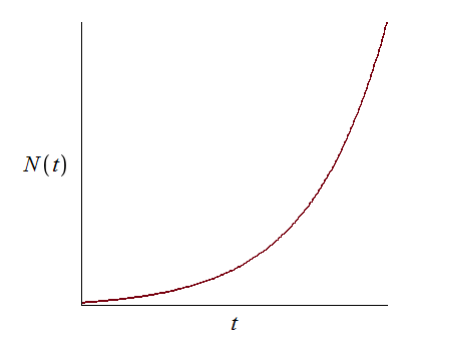
\includegraphics[width=0.7\textwidth,height=\textheight]{./tex2pdf.-cd896adee9a74d13/image/1.png}
\caption{Эволюция популяции жертв и хищников в модели
Лотки-Вольтерры}\label{fig:001}
}
\end{figure}

Математический анализ этой (жесткой) модели показывает, что имеется
стационарное состояние (\(A\) на рис. \ref{fig:001}), всякое же другое
начальное состояние (\(B\)) приводит к периодическому колебанию
численности как жертв, так и хищников, так что по прошествии некоторого
времени система возвращается в состояние \(B\). Стационарное состояние
системы (-\ref{eq:02}) (положение равновесия, не зависящее от времени
решение) будет в точке: \(x_0=\frac{c}{d}\), \(y_0=\frac{a}{b}\).Если
начальные значения задать в стационарном состоянии \(x(0)=x_0\),
\(y(0)=y_0\), в любой момент времени численность популяций изменяться не
будет. При малом отклонении от положения равновесия численности как
хищника, так и жертвы с течением времени не возвращаются к равновесным
значениям, а совершают периодические колебания вокруг стационарной точки
{[}3{]}.

\hypertarget{ux432ux44bux43fux43eux43bux43dux435ux43dux438ux435-ux43bux430ux431ux43eux440ux430ux442ux43eux440ux43dux43eux439-ux440ux430ux431ux43eux442ux44b}{%
\chapter{Выполнение лабораторной
работы}\label{ux432ux44bux43fux43eux43bux43dux435ux43dux438ux435-ux43bux430ux431ux43eux440ux430ux442ux43eux440ux43dux43eux439-ux440ux430ux431ux43eux442ux44b}}

\begin{enumerate}
\def\labelenumi{\arabic{enumi}.}
\item
  Задание в лабораторной работе выполняется по вариантам. Вариант
  расчитывается как номер остаток от деления номера студенческого билета
  на число заданий + 1. Таким образом, мой вариант \textbf{10}:
  1032201739 \% 70 + 1.
\item
  По моему варианту \(x\) - число хищников, а \(y\) - число жертв,
  \(a\), \(d\) - коэффициенты смертности, \(b\), \(c\) - коэффициенты
  прироста популяции. Сопоставляя общий вид системы(-\ref{eq:02}) и
  систему из моего варианта (-\ref{eq:01}) можем определть коэффициенты:
  \(a=0.22\), \(b=0.051\), \(c=0.33\), \(d=0.041\).
\item
  Напишем код для построения графика зависимости численности хищников от
  численности жертв, а также графиков изменения численности хищников и
  численности жертв на Julia:
\end{enumerate}

\begin{verbatim}
#подключаем модули
using Plots
using DifferentialEquations

#задаем начальные условия
const x0 = 3
const y0 = 8

#состояние системы 
u0 = [x0, y0]
#отслеживаемый промежуток времени
time = [0.0, 30.0] 

#задаем константы согласно варианту 
a = 0.22
b = 0.051
c = 0.33
d = 0.041

#сама система 
function M!(du, u, p, t)
    du[1] = -a*u[1]+b*u[1]*u[2]
    du[2] = c*u[2]-d*u[1]*u[2]
end

prob = ODEProblem(M!, u0, time)
sol = solve(prob, saveat=0.05)

const X = Float64[]
const Y = Float64[]

for u in sol.u
    x, y = u
    push!(X,x)
    push!(Y,y)
end
 
#постреоние графиков 
plt1 = plot(
    dpi = 300,
    size = (700,500),
    title ="Изменение численности хищников и численности жертв"
)

plot!(
    plt1,
    sol.t,
    X,
    color =:red,
    label ="Численность хищников"
)

plot!(
    plt1,
    sol.t,
    Y,
    color =:blue,
    label ="Численность жертв"
)

savefig(plt1, "first.png")

plt2 = plot(
    dpi = 300,
    size = (700,500),
    title ="График зависимости численностей"
)

plot!(
    plt2,
    Y,
    X,
    color =:red,
    label ="Зависимость численности хищников от численности жертв"
)

savefig(plt2, "first_php.png")
\end{verbatim}

\begin{enumerate}
\def\labelenumi{\arabic{enumi}.}
\setcounter{enumi}{3}
\tightlist
\item
  Напишем код ддля построения графика зависимости численности хищников
  от численности жертв, а также графиков изменения численности хищников
  и численности жертв на OpenModelica:
\end{enumerate}

\begin{verbatim}
model lab05

 Real x(start=3.0);
 Real y(start=8.0);
 constant Real a = 0.22;
 constant Real b = 0.051;
 constant Real c = 0.33;
 constant Real d = 0.041;
  
equation
  der(x) = -a*x+b*x*y;
  der(y) = c*y-d*x*y;

end lab05;
\end{verbatim}

\begin{enumerate}
\def\labelenumi{\arabic{enumi}.}
\setcounter{enumi}{4}
\tightlist
\item
  Видим результаты, полученные с помощью Julia: график зависимости
  численности хищников от численности жертв (рис. \ref{fig:002}) и
  графики изменения численности хищников и численности жертв (рис.
  \ref{fig:003}).
\end{enumerate}

\begin{figure}
\hypertarget{fig:002}{%
\centering
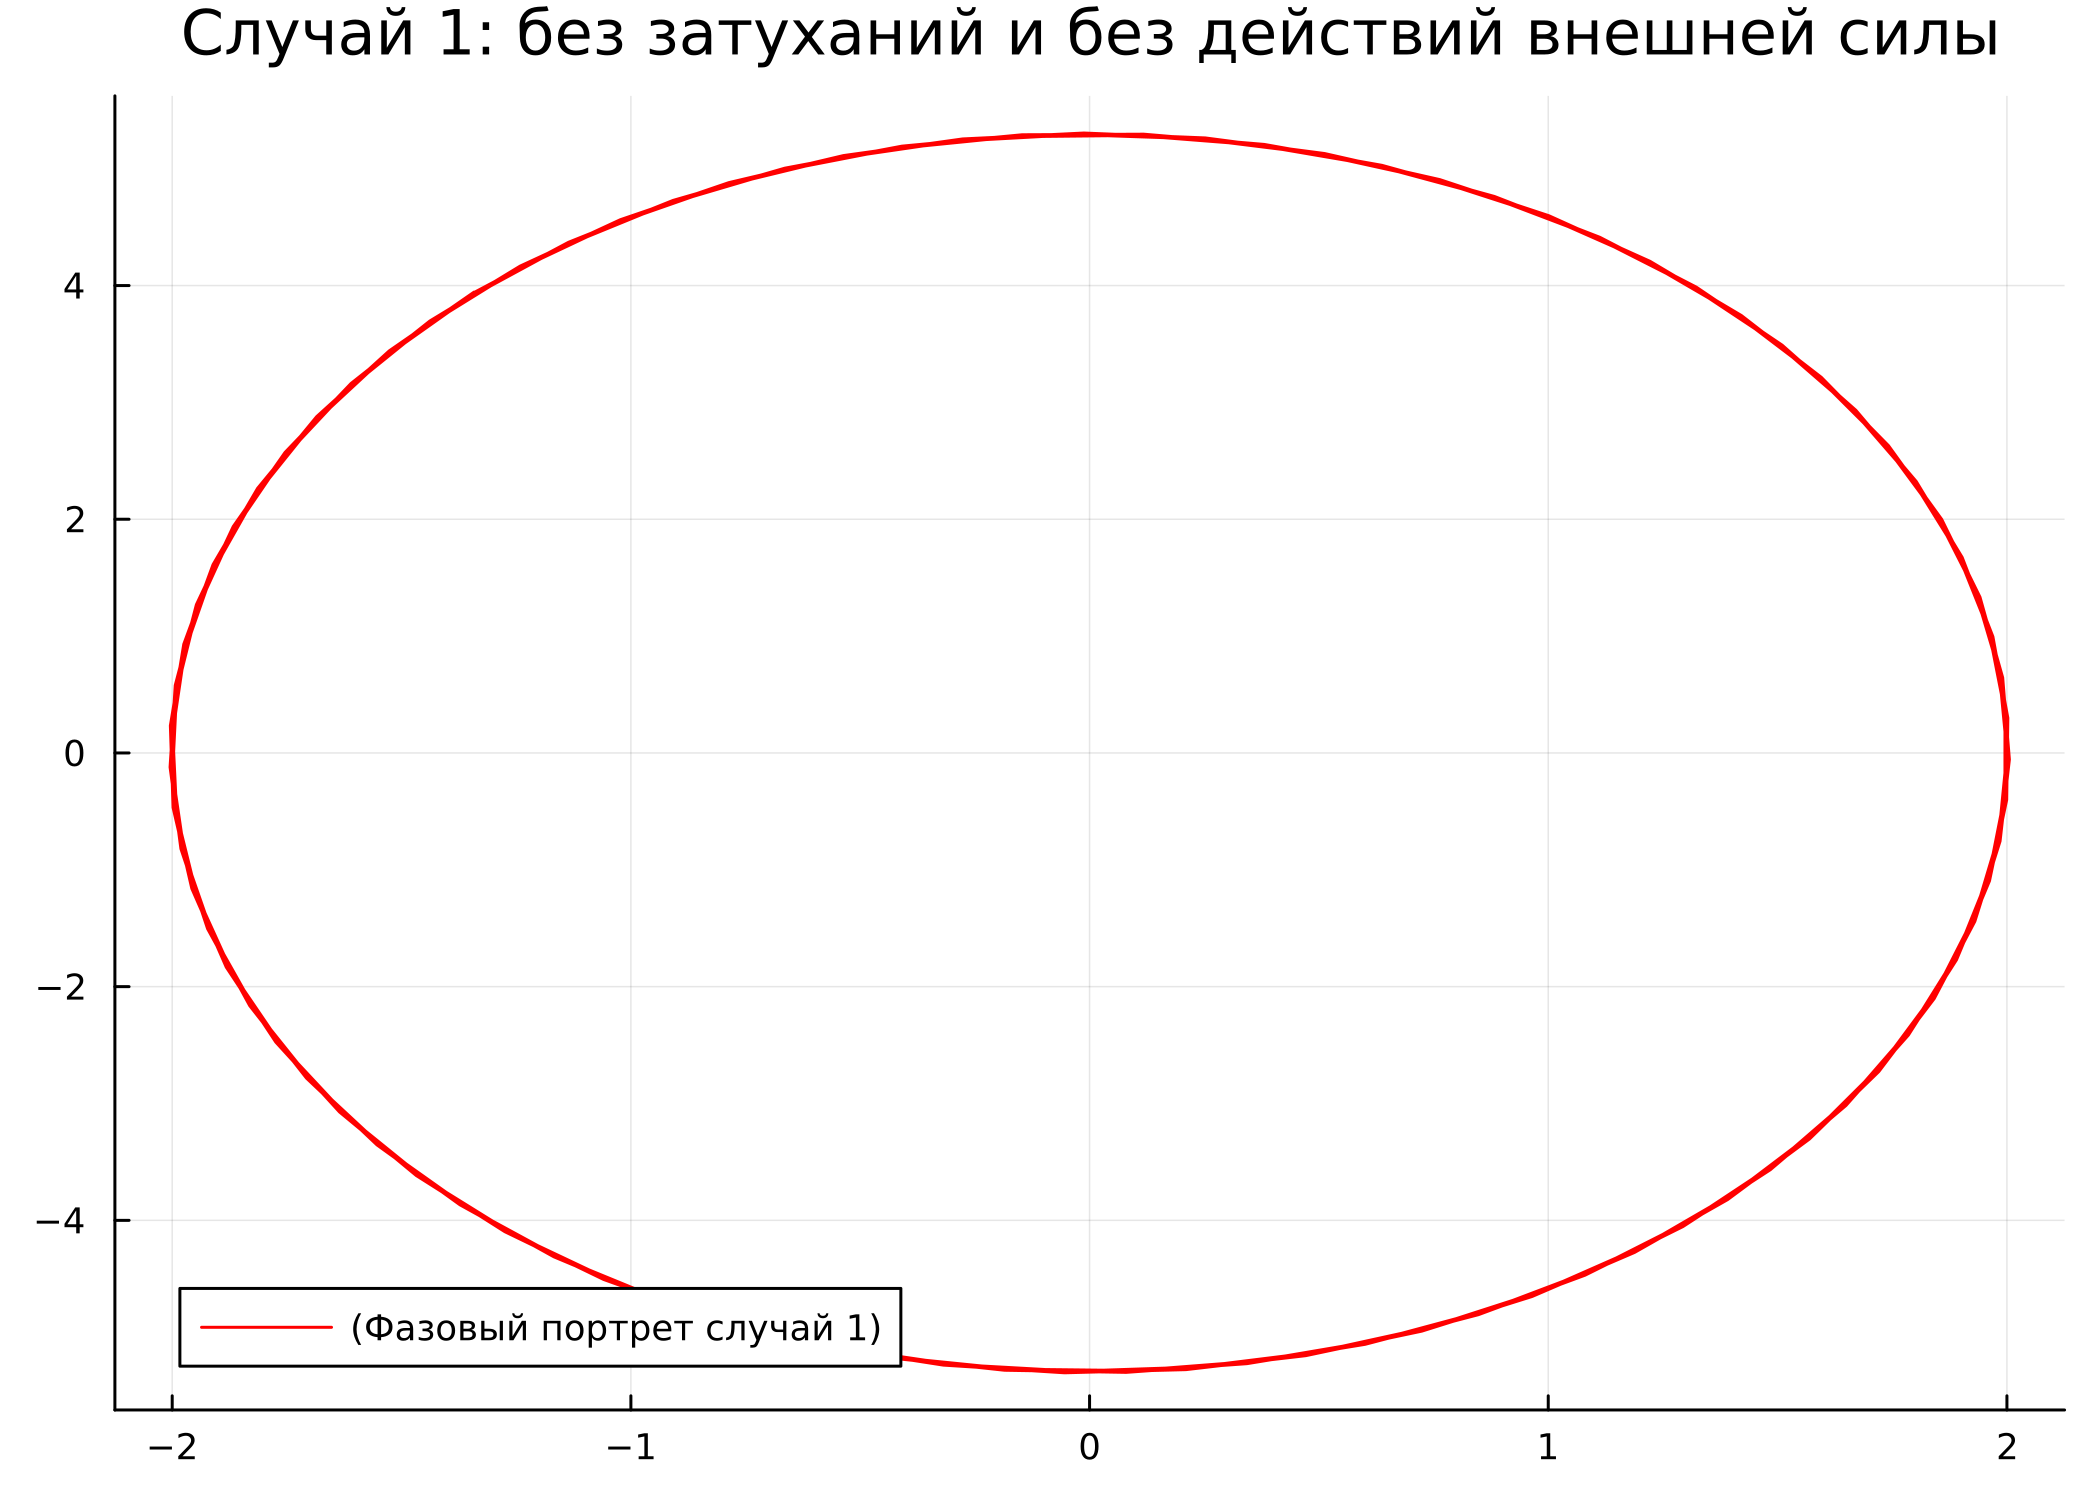
\includegraphics[width=0.7\textwidth,height=\textheight]{./tex2pdf.-cd896adee9a74d13/image/first_php.png}
\caption{График зависимости численности хищников от численности жертв
(Julia)}\label{fig:002}
}
\end{figure}

\begin{figure}
\hypertarget{fig:003}{%
\centering
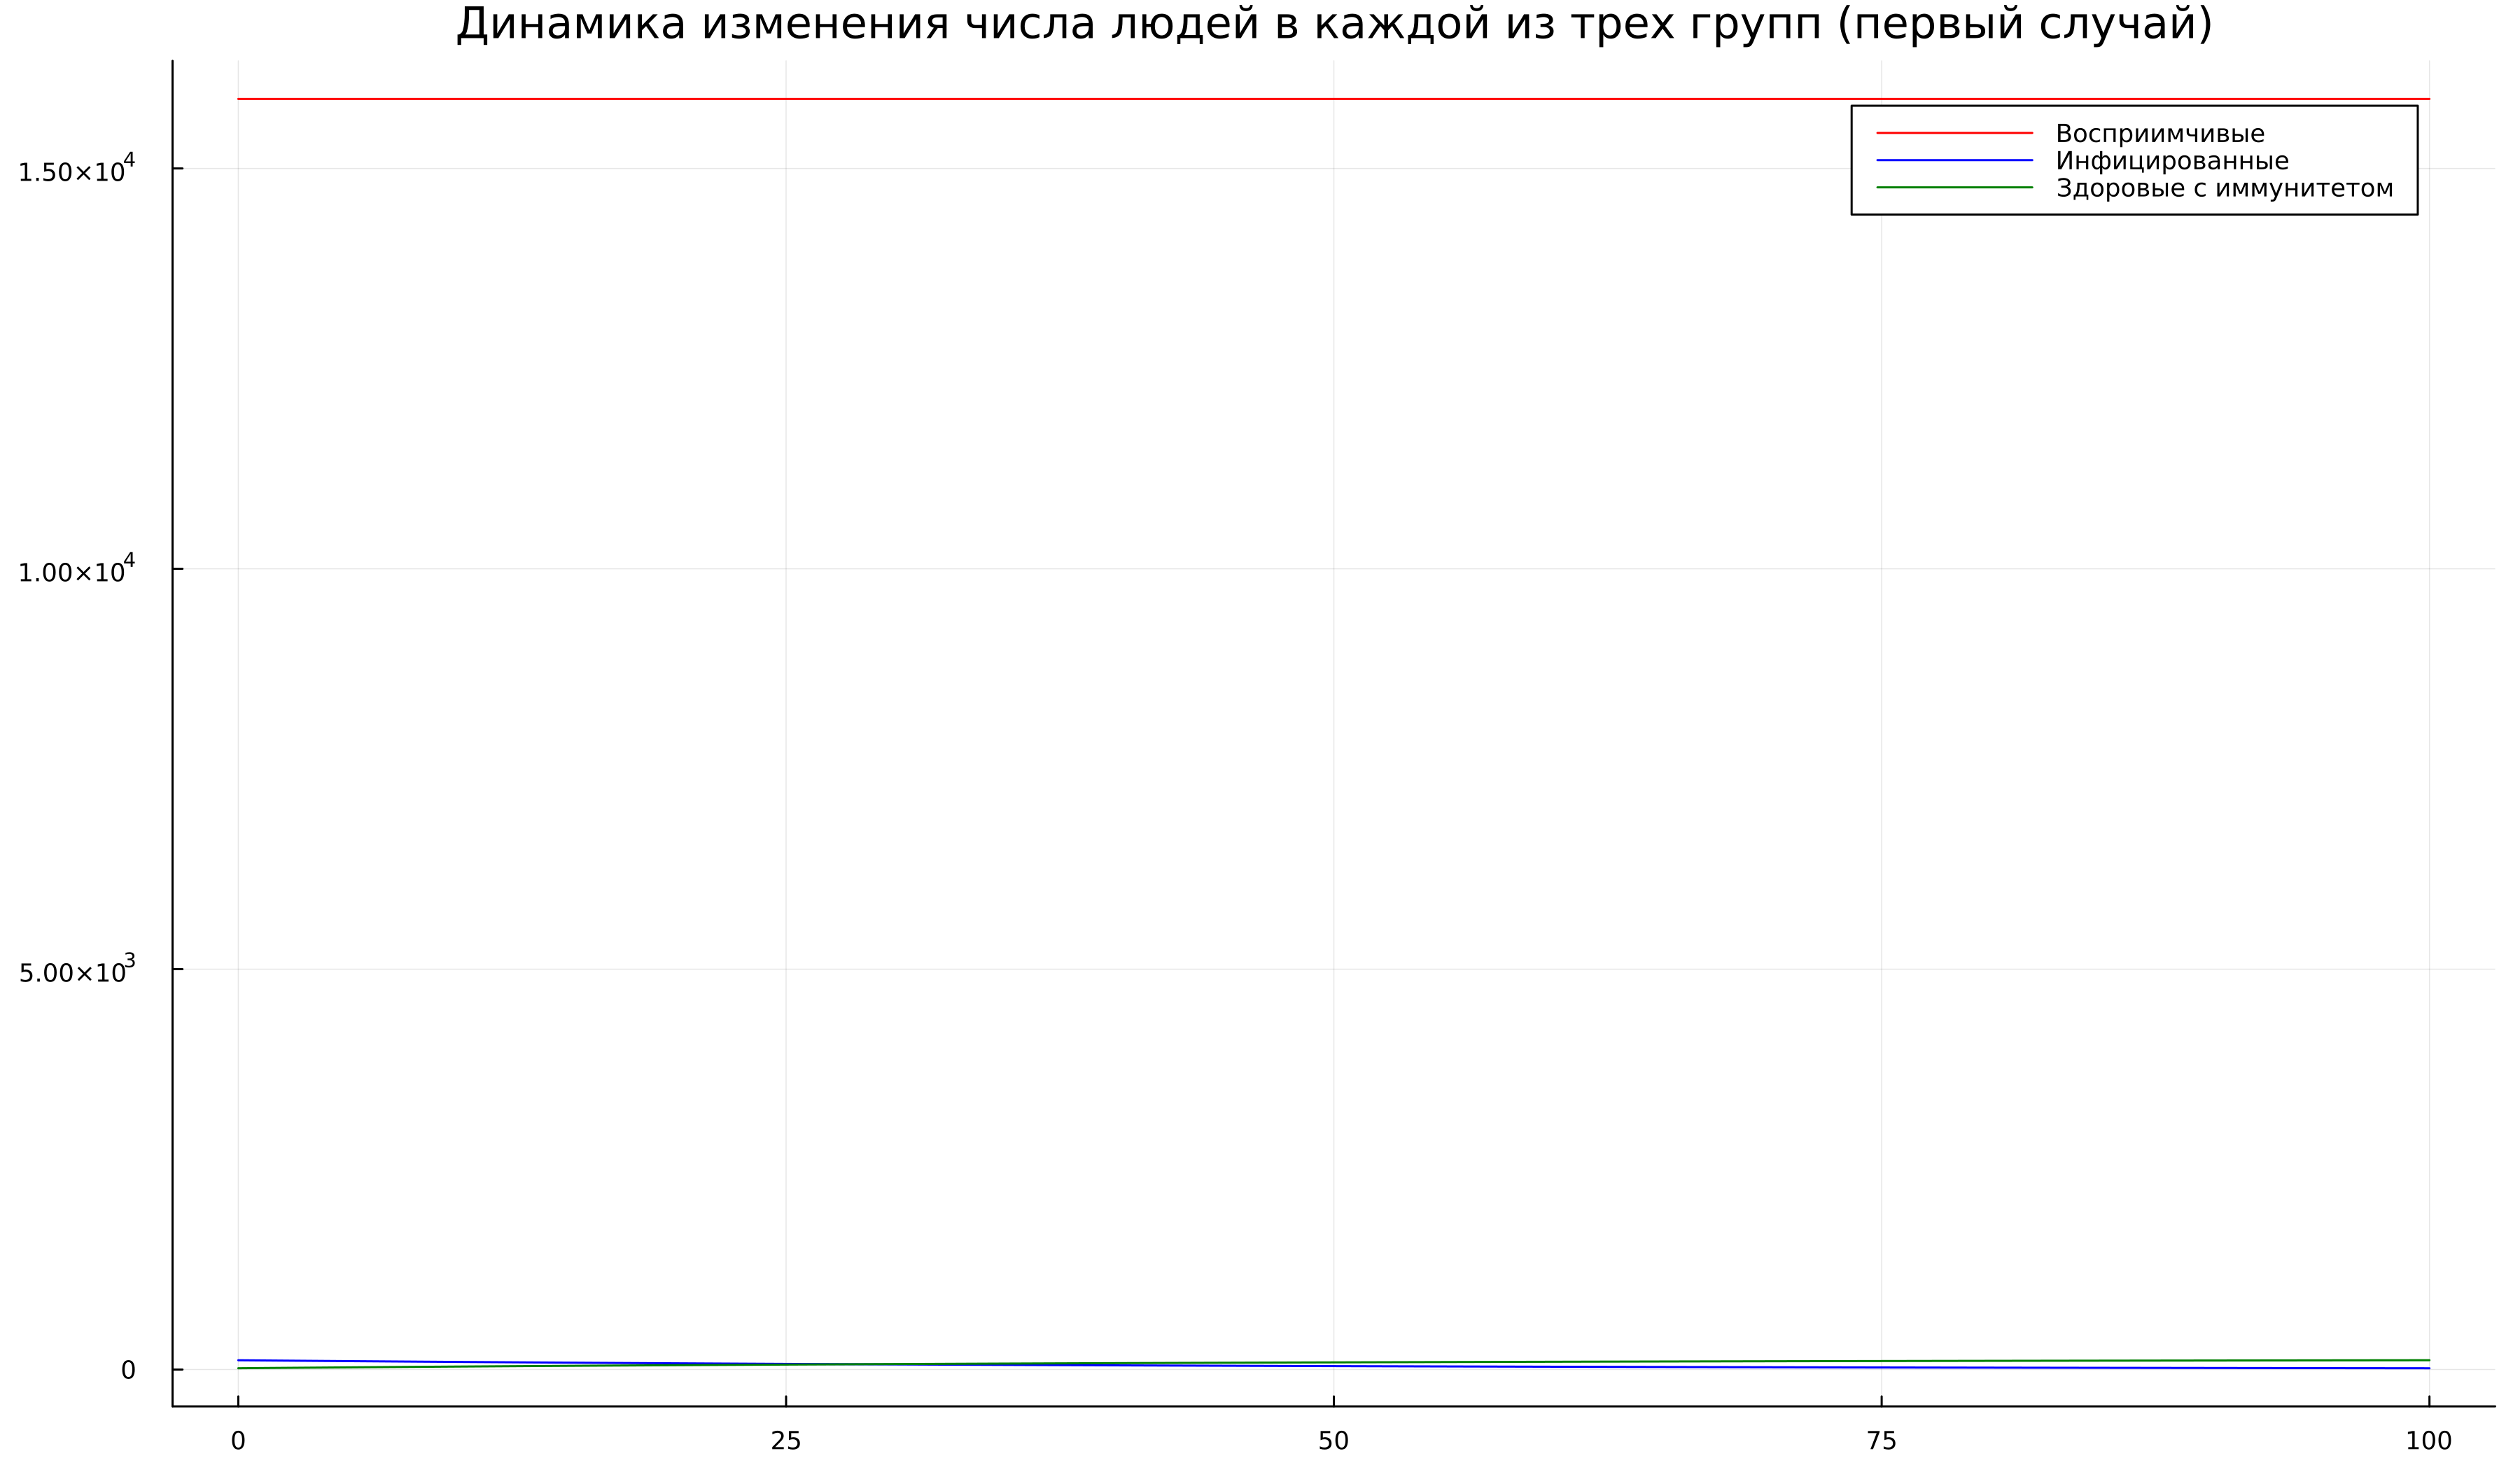
\includegraphics[width=0.7\textwidth,height=\textheight]{./tex2pdf.-cd896adee9a74d13/image/first.png}
\caption{График изменения численности хищников и численности жертв
(Julia)}\label{fig:003}
}
\end{figure}

\begin{enumerate}
\def\labelenumi{\arabic{enumi}.}
\setcounter{enumi}{5}
\tightlist
\item
  Видим результаты, полученные с помощью OpenModelica: график
  зависимости численности хищников от численности жертв (рис.
  \ref{fig:004}) и графики изменения численности хищников и численности
  жертв (рис. \ref{fig:005}).
\end{enumerate}

\begin{figure}
\hypertarget{fig:004}{%
\centering
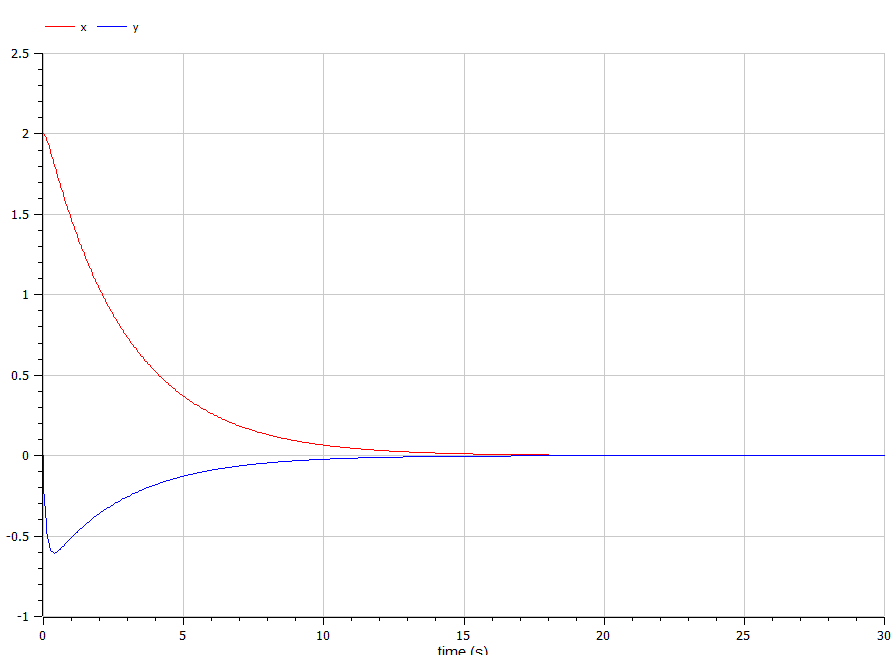
\includegraphics[width=0.7\textwidth,height=\textheight]{./tex2pdf.-cd896adee9a74d13/image/second_om.png}
\caption{График зависимости численности хищников от численности жертв
(OpenModelica)}\label{fig:004}
}
\end{figure}

\begin{figure}
\hypertarget{fig:005}{%
\centering
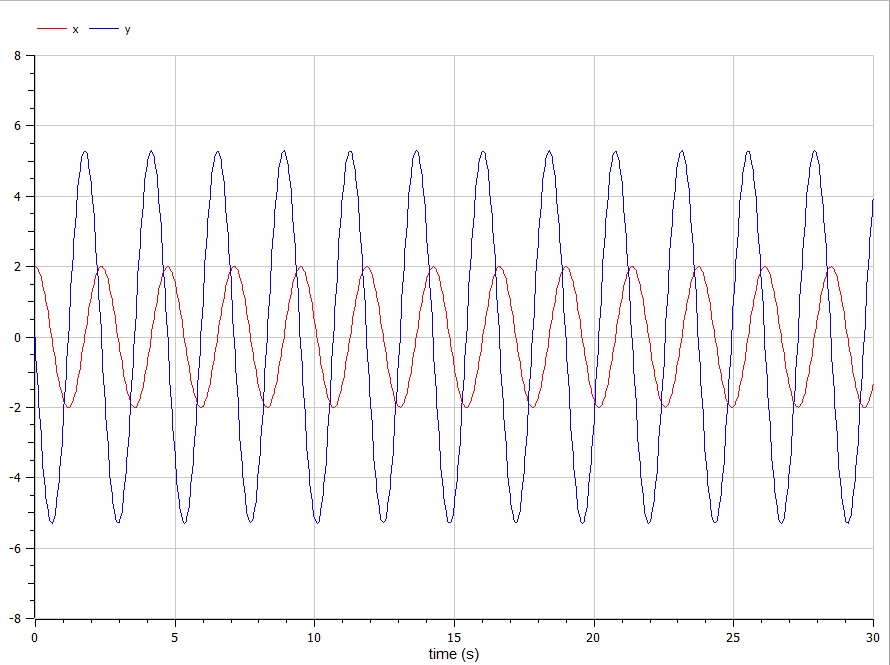
\includegraphics[width=0.7\textwidth,height=\textheight]{./tex2pdf.-cd896adee9a74d13/image/first_om.png}
\caption{График изменения численности хищников и численности жертв
(OpenModelica)}\label{fig:005}
}
\end{figure}

\begin{enumerate}
\def\labelenumi{\arabic{enumi}.}
\setcounter{enumi}{6}
\item
  Теперь на нужно найти стационарное сосотояние. Оно, как уже было
  описано выше, находится как \(x_0=\frac{a}{b}\), \(y_0=\frac{c}{d}\).
  Удобнее всего будет сразу посчитать его в Julia, поэтому напишем код
  на Julia, в котором будет считаться и выводиться на экран стационарное
  состоояние. Кроме того, если стационарное состояние посчитано верно и
  подставлено в начальные значения численности хищников и жертв, графики
  изменения численности хищников и численности жертв будут выглядеть как
  две параллельные прямые, а график зависимости численности хищников от
  численности жертв будет точкой. Для проверки правильности подставим
  полученное стационарное в наш код на Julia.
\item
  Напишем код для расчета и проверки стационарного состояния на Julia:
\end{enumerate}

\begin{verbatim}
#подключаем модули
using Plots
using DifferentialEquations

#задаем коэффициенты согласно варианту 
a = 0.22
b = 0.051
c = 0.33
d = 0.041

#задаем начальные условия
x0 = c / d
y0 = a / b

#состояние системы 
u0 = [x0, y0]
#отслеживаемый промежуток времени
time = [0.0, 120.0] 

print("x0 = ")
println(x0)
print("y0 = ")
println(y0)

#сама система 
function M!(du, u, p, t)
    du[1] = -a*u[1]+b*u[1]*u[2]
    du[2] = c*u[2]-d*u[1]*u[2]
end

prob = ODEProblem(M!, u0, time)
sol = solve(prob, saveat=0.05)

const X = Float64[]
const Y = Float64[]

for u in sol.u
    x, y = u
    push!(X,x)
    push!(Y,y)
end
 
#постреоние графиков 
plt1 = plot(
    dpi = 300,
    size = (700,500),
    title ="Изменение численности хищников и численности жертв"
)

plot!(
    plt1,
    sol.t,
    X,
    color =:red,
    label ="Численность хищников"
)

plot!(
    plt1,
    sol.t,
    Y,
    color =:blue,
    label ="Численность жертв"
)

savefig(plt1, "second.png")

plt2 = plot(
    dpi = 300,
    size = (700,500),
    title ="График зависимости численностей"
)

plot!(
    plt2,
    Y,
    X,
    color =:red,
    label ="Зависимость численности хищников от численности жертв"
)

savefig(plt2, "second_php.png")
\end{verbatim}

\begin{enumerate}
\def\labelenumi{\arabic{enumi}.}
\setcounter{enumi}{8}
\tightlist
\item
  Посмотрим на результаты, полученные с помощью Julia для расчета (рис.
  \ref{fig:006}) и проверки (рис. {[}\ref{fig:007}-\ref{fig:008}{]})
  стационарного состояния. Видим, что полученный результат верен.
  Фазовый портрет физуально выглядит не точкой, однако, если мы
  посмотрим на значения на осях, видим, что числа очень малы. Так, это
  просто погрешность вычислений, фактически это точка.
\end{enumerate}

\begin{figure}
\hypertarget{fig:006}{%
\centering
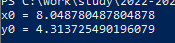
\includegraphics[width=0.7\textwidth,height=\textheight]{./tex2pdf.-cd896adee9a74d13/image/st_p.png}
\caption{Стационарное состояние}\label{fig:006}
}
\end{figure}

\begin{figure}
\hypertarget{fig:007}{%
\centering
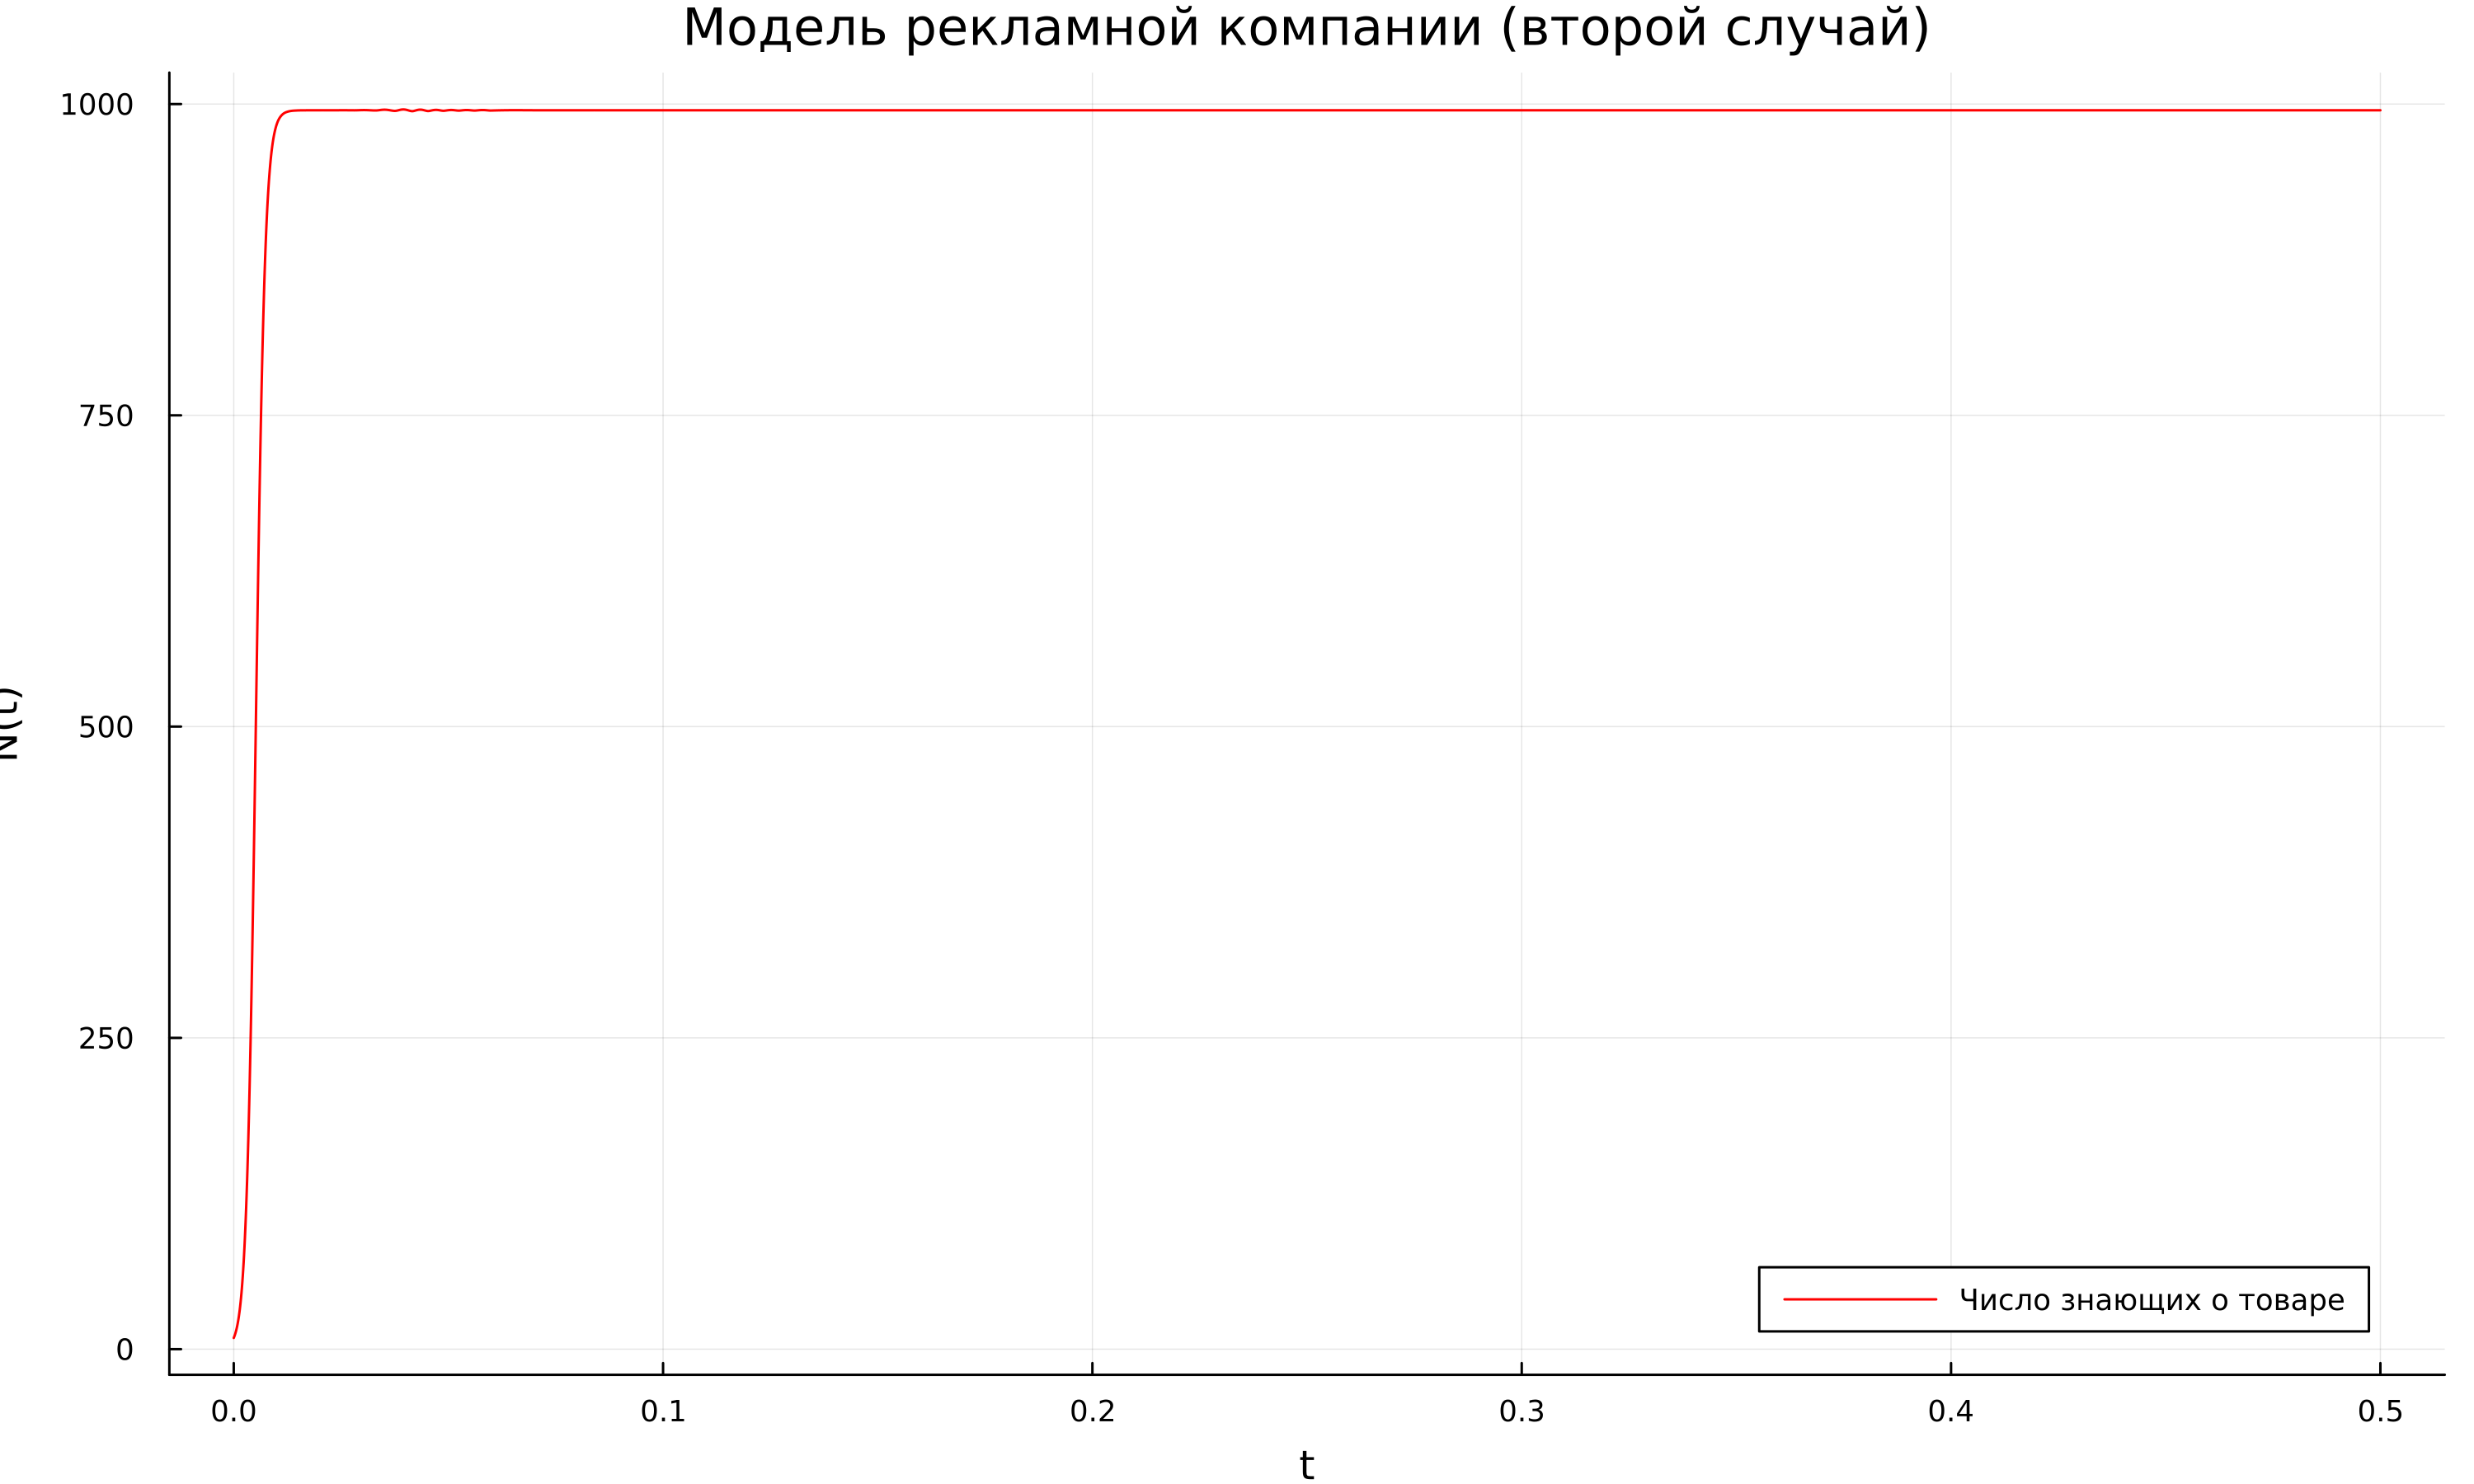
\includegraphics[width=0.7\textwidth,height=\textheight]{./tex2pdf.-cd896adee9a74d13/image/second.png}
\caption{Графики изменения численности жертв с начальными состояниями в
стационарных точках}\label{fig:007}
}
\end{figure}

\begin{figure}
\hypertarget{fig:008}{%
\centering
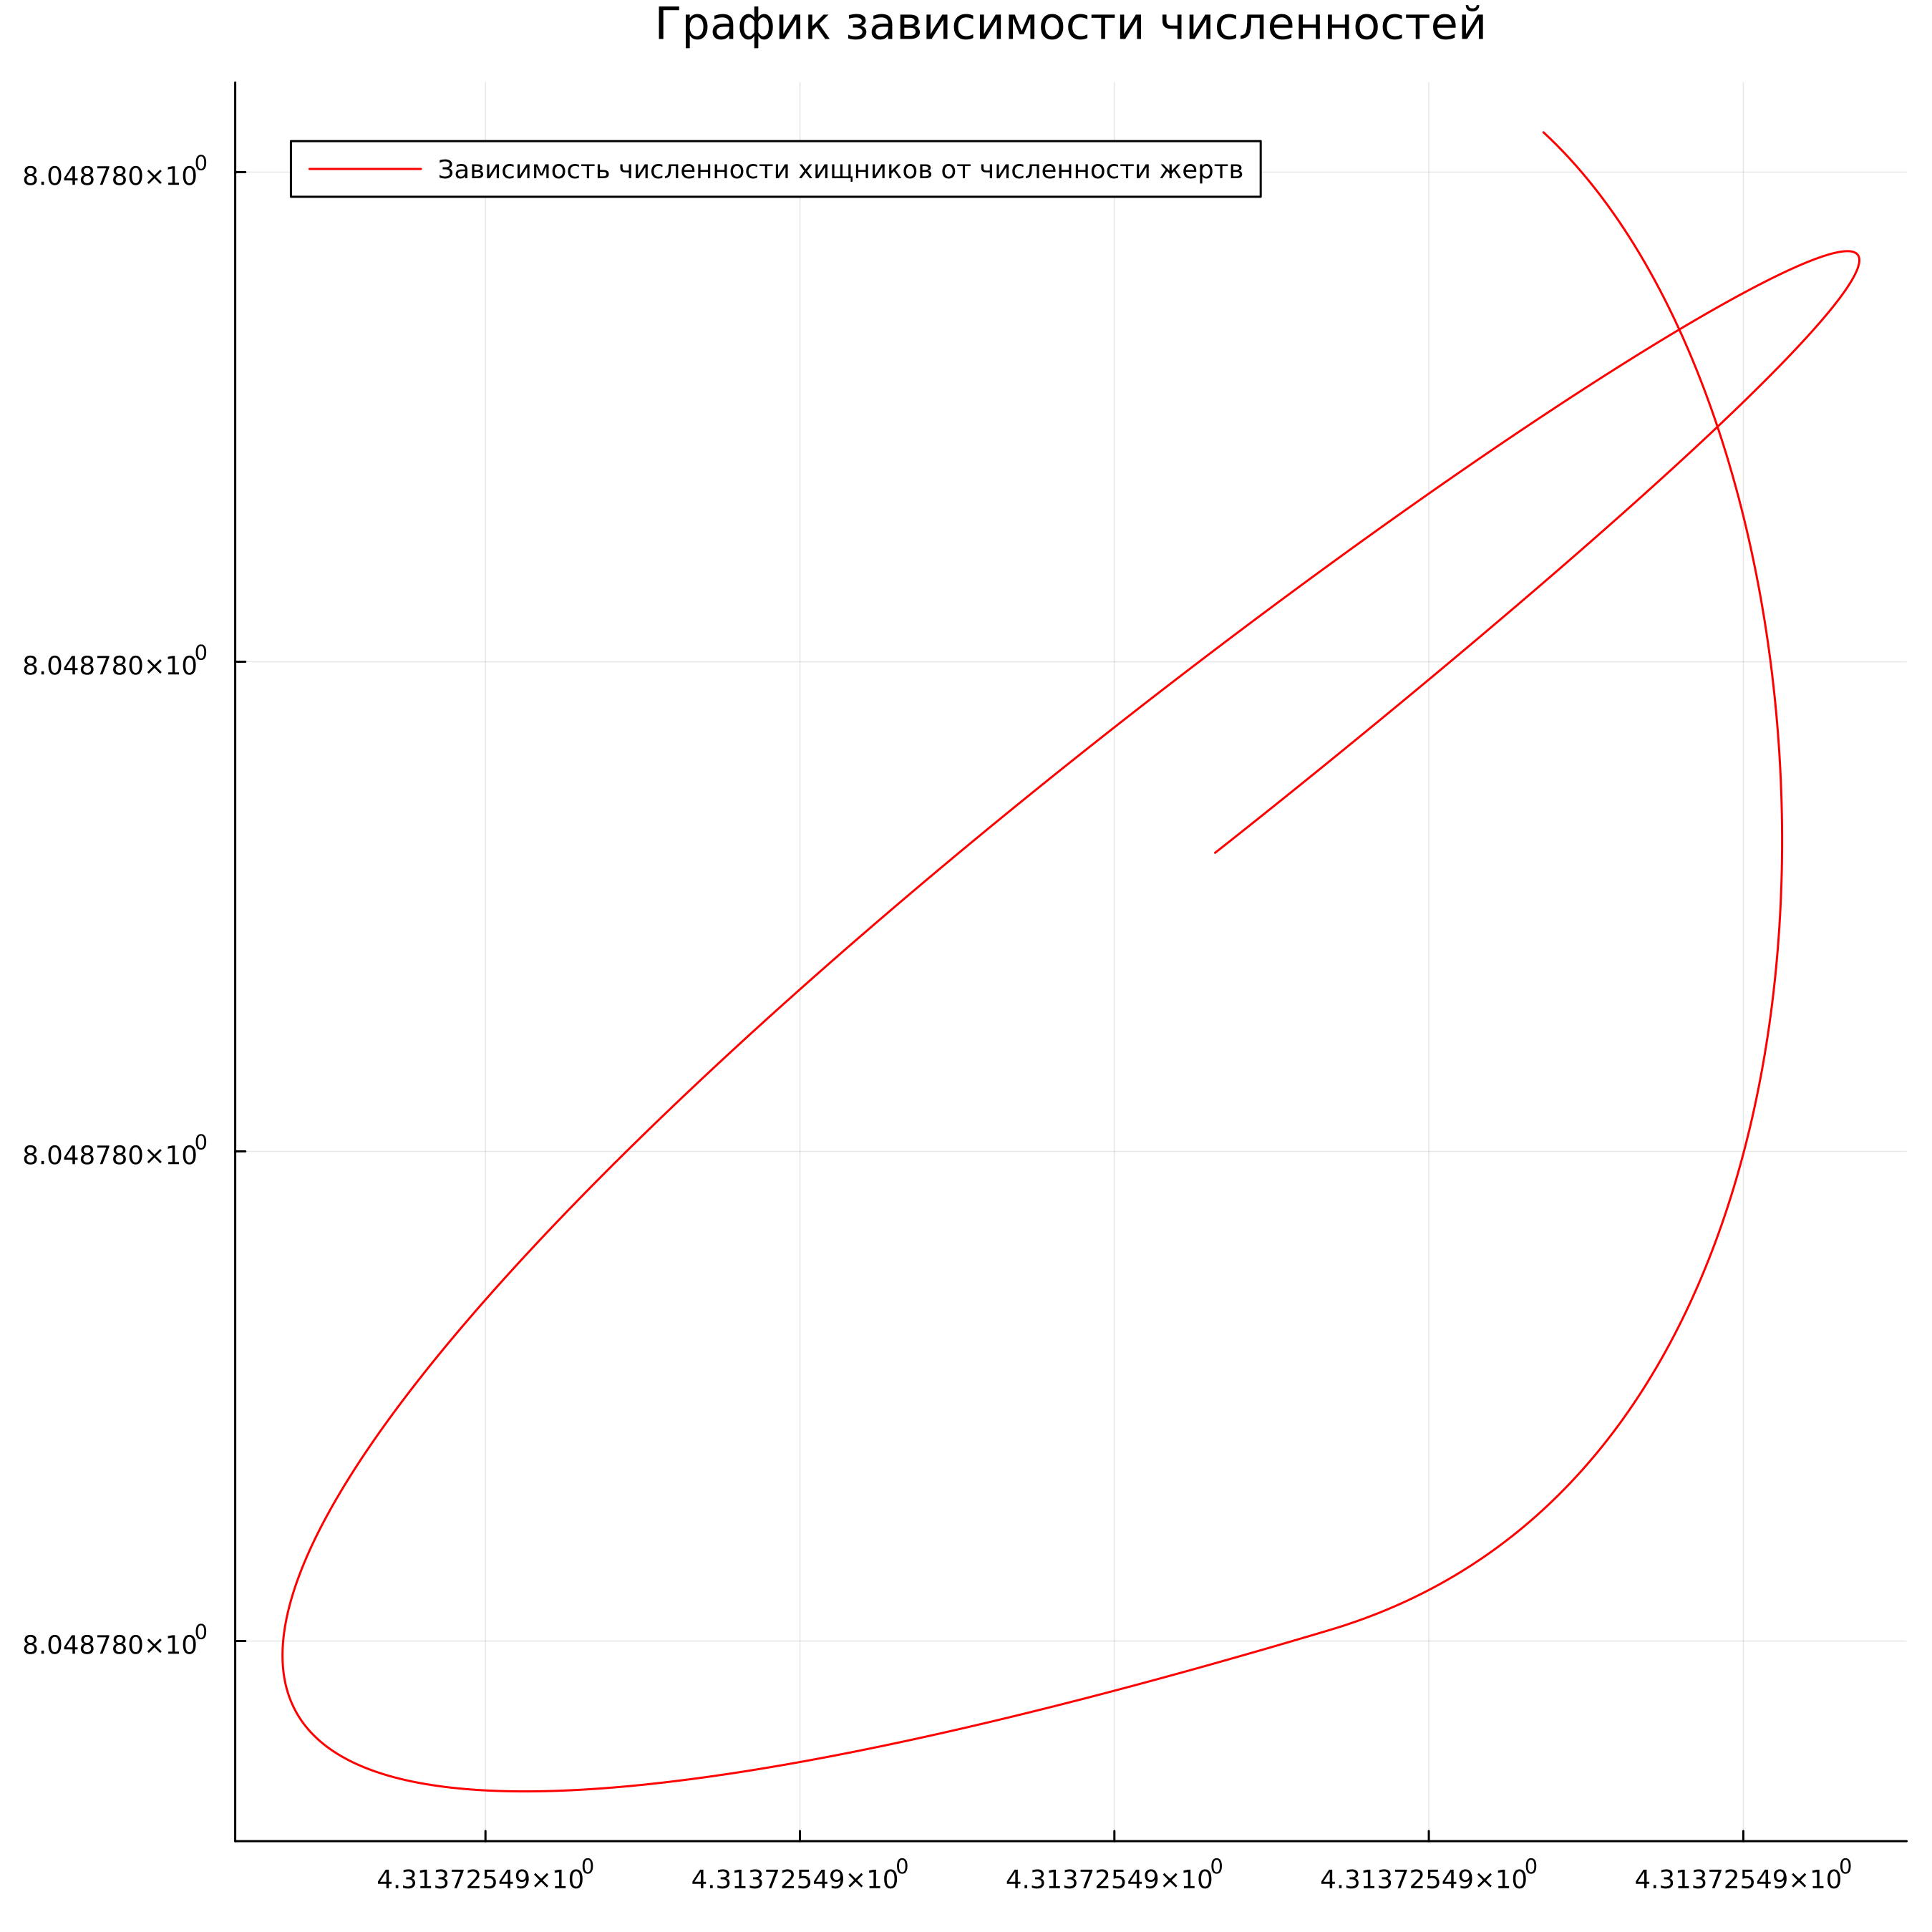
\includegraphics[width=0.7\textwidth,height=\textheight]{./tex2pdf.-cd896adee9a74d13/image/second_php.png}
\caption{График зависимости численности жертв с начальными состояниями в
стационарных точках}\label{fig:008}
}
\end{figure}

\hypertarget{ux432ux44bux432ux43eux434ux44b}{%
\chapter{Выводы}\label{ux432ux44bux432ux43eux434ux44b}}

Я рассмотрела простейшую модель взаимодействия двух видов типа «хищник —
жертва» - модель Лотки-Вольтерры. Выполнила задание согласно варианту:
построила график зависимости численности хищников от численности жертв,
а также графики изменения численности хищников и численности жертв при
заданных начальных условиях, нашла стационарное сосотояние системы.

\hypertarget{ux441ux43fux438ux441ux43eux43a-ux43bux438ux442ux435ux440ux430ux442ux443ux440ux44b}{%
\chapter*{Список
литературы}\label{ux441ux43fux438ux441ux43eux43a-ux43bux438ux442ux435ux440ux430ux442ux443ux440ux44b}}
\addcontentsline{toc}{chapter}{Список литературы}

\hypertarget{refs}{}
\begin{CSLReferences}{0}{0}
\leavevmode\vadjust pre{\hypertarget{ref-key-1}{}}%
\CSLLeftMargin{1. }%
\CSLRightInline{{Уравнение Лотки-Вольтерры для моделирования
хищничества} {[}Электронный ресурс{]}. Про уравнения - легко, 2023. URL:
\url{https://al-shell.ru/articles/uravnenie-lotki-volterry-dlya-modelirovaniya-hischnichestva/}.}

\leavevmode\vadjust pre{\hypertarget{ref-key-2}{}}%
\CSLLeftMargin{2. }%
\CSLRightInline{{Компьютерная модель "хищник-жертва"} {[}Электронный
ресурс{]}. Электронный научно-практический журнал «Современные научные
исследования и инновации», 2017. URL:
\url{https://web.snauka.ru/issues/2017/01/77530}.}

\leavevmode\vadjust pre{\hypertarget{ref-key-3}{}}%
\CSLLeftMargin{3. }%
\CSLRightInline{{Лабораторная работа №5} {[}Электронный ресурс{]}.
Российский университет дружбы народов, 2023. URL:
\url{https://esystem.rudn.ru/pluginfile.php/1971733/mod_resource/content/2/Лабораторная\%20работа\%20№\%204.pdf}.}

\end{CSLReferences}

\printbibliography

\end{document}
